%% ================================================================
%% IEEE Conference Paper — paper.tex (Master 6+ Page Submission)
%% Title: Centralized vs. Decentralized Distributed Training:
%%        A Head-to-Head Empirical Comparison of Downpour SGD and Gossip SGD
%% ================================================================

\documentclass[conference]{IEEEtran}

\usepackage{cite}
\usepackage{amsmath,amssymb,amsfonts}
\usepackage{graphicx}
\usepackage{textcomp}
\usepackage{xcolor}
\usepackage{booktabs}
\usepackage{url}
\usepackage{array}
\usepackage{multirow}

\begin{document}

% ================================================================
%  TITLE
% ================================================================
\title{Centralized vs.\ Decentralized Distributed Training:\\
A Head-to-Head Empirical Comparison of Downpour SGD\\
and Gossip SGD}

\author{
  \IEEEauthorblockN{Alok Jha}
  \IEEEauthorblockA{
    Department of Computer Science and Engineering\\
    {Indian Institute of Information Technology, Pune, India}\\
    Email: alokj0409@gmail.com}
}

\maketitle

% ================================================================
%  ABSTRACT
% ================================================================
\begin{abstract}
Distributed Stochastic Gradient Descent (SGD) is foundational to large-scale deep learning. Two dominant paradigms exist: the \emph{centralized Parameter Server} (PS) approach, exemplified by Downpour SGD, and \emph{decentralized peer-to-peer} weight averaging, exemplified by Gossip SGD. Despite theoretical maturity, rigorous empirical comparisons under identical network constraints, bandwidth caps, and exchange frequencies remain sparse. This paper presents a complete head-to-head empirical study implemented from scratch using PyTorch~2.13, gRPC~1.83, and Protocol Buffers in a Docker-based multi-process simulation environment on an Intel Core i5-12450H workstation (16\,GB RAM, CPU-only). Both systems train a four-layer Convolutional Neural Network (CNN, 586,250 parameters) on CIFAR-10 across five experimental dimensions: baseline convergence quality, software network latency simulation ($0\to 100$\,ms), bandwidth throttling ($100$\,Mbps), gossip exchange interval sweeps ($\text{gossip\_every} \in \{1,5,10\}$), worker scalability ($N \in \{2,4\}$), peak single-node bandwidth strain, and live fault-injection resilience.

Key empirical findings: (1)~Downpour SGD completes baseline three-epoch training in $166.98$\,s versus $258.01$\,s for Gossip SGD ($1.54\times$ faster) and generates half the baseline payload ($11.0$\,GB vs.\ $22.0$\,GB). (2)~Under an artificial $100$\,Mbps network bandwidth cap, Decentralized Gossip SGD outpaces Centralized Downpour SGD by $15.45$\,s ($159.69$\,s vs.\ $175.14$\,s) due to Parameter Server NIC bottlenecking ($N\times\text{payload}$). (3)~Optimizing gossip exchange frequency ($\text{gossip\_every}=5$) yields a $1.72\times$ wall-clock speedup ($80.29$\,s vs.\ $46.57$\,s) and a $5\times$ payload reduction ($7.32$\,GB to $1.46$\,GB) while preserving convergence. (4)~At $N=4$ workers, Gossip SGD achieves superior parallel efficiency ($57.45\%$ vs.\ $51.87\%$). (5)~Gossip SGD tolerates worker crashes via autonomous peer pruning without training disruption, whereas Downpour SGD halts irreversibly upon Parameter Server failure. These measurement-backed findings align empirical systems behavior with NeurIPS 2017 D-PSGD theoretical principles.
\end{abstract}

\begin{IEEEkeywords}
Distributed Machine Learning, Distributed SGD, Downpour SGD, Gossip SGD, Parameter Server, Fault Tolerance, Decentralized Optimization, gRPC, Peer-to-Peer Systems, Network Latency, Bandwidth Throttling
\end{IEEEkeywords}

% ================================================================
%  I. INTRODUCTION
% ================================================================
\section{Introduction}

The computational demands of modern deep-learning models have consistently outpaced single-machine capacity. Training large neural networks requires distributing gradient computation across multiple worker processes or physical nodes~\cite{dean2012large}. This distribution introduces a fundamental architectural choice: \emph{how} should model parameters be maintained, communicated, and updated across workers?

\subsection{Centralized Parameter Server}
The centralized paradigm, formalized in DistBelief and Downpour SGD~\cite{dean2012large}, designates one or more Parameter Server (PS) nodes as the authoritative keeper of global model weights. Worker nodes asynchronously push locally-computed gradients to the PS, which applies an adaptive update rule (Adagrad~\cite{duchi2011adaptive}) and serves the latest weights on demand. This architecture is simple and enables fast early convergence, but concentrates network bandwidth and introduces a single point of failure at the PS.

\subsection{Decentralized Gossip-Based SGD}
Decentralized approaches eliminate the central server entirely~\cite{lian2017can}. In Gossip SGD, each worker maintains its own local model copy, trains on a local data shard, and periodically exchanges model weights with a randomly selected peer. Both sides average their weights after exchange, driving the cluster toward parameter consensus. Without a central bottleneck, this architecture scales more gracefully and tolerates node failures without global disruption~\cite{blot2016gossip}.

\subsection{Motivation and Research Questions}
Despite theoretical progress, systems-level empirical evaluation under controlled network latency, bandwidth throttling, and exchange frequency parameters is rarely reported. Most published studies evaluate one paradigm in isolation or omit peak per-worker network overhead. This paper addresses four fundamental research questions:
\begin{enumerate}
    \item \textbf{RQ1 (Latency Crossover)}: Under what network latency $\Delta t$ does Decentralized Gossip SGD outpace Centralized Downpour SGD?
    \item \textbf{RQ2 (Bandwidth Bottleneck)}: How do link capacity constraints ($100\text{ Mbps}$) impact single-node Parameter Server bottlenecks vs.\ P2P load distribution?
    \item \textbf{RQ3 (Communication Interval)}: What is the optimal \texttt{gossip\_every} interval ($1, 5, 10$) to minimize wall-clock runtime without sacrificing model convergence?
    \item \textbf{RQ4 (Scalability \& Faults)}: How do parallel speedup $S(N)$ and fault resilience compare across worker counts $N \in \{2, 4\}$?
\end{enumerate}

\subsection{Key Contributions}
This work makes the following concrete contributions:
\begin{enumerate}
    \item A fully functional gRPC/Protobuf implementation of Downpour SGD and Gossip SGD built from scratch in Python/PyTorch.
    \item A Docker Compose simulation environment for reproducible multi-worker deployment on a single host.
    \item A software network simulation engine implementing gRPC interceptors (\texttt{NetworkSimulatorClientInterceptor}) for $0\to 100$\,ms artificial latency and $100$\,Mbps bandwidth throttling.
    \item An empirical evaluation of Gossip communication intervals ($\text{gossip\_every} \in \{1, 5, 10\}$), proving a $1.72\times$ runtime speedup and $5\times$ network traffic drop.
    \item Measurements of peak single-node network strain, parallel speedup $S(N)$, and parallel efficiency $E(N)$ up to $N=4$ workers.
    \item Live fault-injection suite evaluating dynamic peer pruning vs.\ Parameter Server single point of failure (SPOF).
\end{enumerate}

% ================================================================
%  II. BACKGROUND AND RELATED WORK
% ================================================================
\section{Background and Related Work}

\subsection{Downpour SGD and DistBelief}
Dean et al.~\cite{dean2012large} introduced DistBelief and Downpour SGD, where model replicas push gradients to sharded PS nodes. The PS applies Adagrad~\cite{duchi2011adaptive} for adaptive per-parameter learning rates, allowing workers to operate without global synchronization barriers. Li et al.~\cite{li2014scaling} provided scalability analysis of the PS framework, highlighting bandwidth concentration at the server as a limiting factor.

\subsection{Decentralized Optimization (D-PSGD)}
Lian et al.~\cite{lian2017can} formally analyzed Decentralized Parallel SGD (D-PSGD), proving theoretical convergence for non-convex objectives under doubly-stochastic mixing matrices. Jin et al.~\cite{jin2016scale} and Blot et al.~\cite{blot2016gossip} studied gossip-style weight averaging, demonstrating spectral mixing on complete graphs. Nedic and Ozdaglar~\cite{nedic2009distributed} provided foundational theory for distributed subgradient convergence over peer networks.

\subsection{Fault Tolerance in Distributed Deep Learning}
Synchronous all-reduce systems (e.g., Horovod~\cite{sergeev2018horovod}) require all workers in every step, making them highly sensitive to crashes. Asynchronous PS systems handle worker failures gracefully (missing pushes are simply omitted) but lose their entire state on PS failure~\cite{ho2013more}. Gossip systems have the theoretical advantage of no single critical node, a property empirically verified in this work.

% ================================================================
%  III. SYSTEM ARCHITECTURE AND DESIGN
% ================================================================
\section{System Architecture and Design}

\subsection{Model and Dataset Workload}
Both systems train an identical four-layer Convolutional Neural Network (\texttt{CifarCNN}) on CIFAR-10~\cite{krizhevsky2009learning}:
\begin{itemize}
    \item \textbf{Conv Block 1}: Conv2d(3 $\to$ 32, 3$\times$3, pad 1) $\to$ ReLU $\to$ MaxPool(2$\times$2)
    \item \textbf{Conv Block 2}: Conv2d(32 $\to$ 64, 3$\times$3, pad 1) $\to$ ReLU $\to$ MaxPool(2$\times$2)
    \item \textbf{Conv Block 3}: Conv2d(64 $\to$ 64, 3$\times$3, pad 1) $\to$ ReLU $\to$ MaxPool(2$\times$2)
    \item \textbf{FC Layer}: Linear(1024 $\to$ 512) $\to$ ReLU $\to$ Dropout(0.25) $\to$ Linear(512 $\to$ 10)
\end{itemize}
Total trainable parameters: \textbf{586,250}. The 50,000-sample CIFAR-10 training set is partitioned into $N$ contiguous, disjoint shards. Data augmentation includes random horizontal flip and random crop (size 32, padding 4).

\subsection{Communication Layer and Interceptor Engine}
All inter-process communication uses \textbf{gRPC 1.83} over Protocol Buffers 3 (\texttt{proto3}). Raw \texttt{float32} tensors are serialized via \texttt{numpy.tobytes()} into the \texttt{bytes} data field of each \texttt{TensorData} message and deserialized with \texttt{numpy.frombuffer}. The maximum gRPC message size is configured to 100\,MB to accommodate full model state dicts ($\approx 2.34$\,MB per tensor payload).

Network simulation is implemented using a custom gRPC client interceptor (\texttt{NetworkSimulatorClientInterceptor}):
\begin{equation}
    t_{\text{delay}} = \frac{\text{latency\_ms}}{1000} + \frac{\text{payload\_bytes} \times 8}{\text{bandwidth\_bps}}
\end{equation}

\subsection{Downpour SGD Architecture}
The Parameter Server (\texttt{server.py}) exposes two RPCs:
\begin{itemize}
    \item \texttt{rpc PushGradients(GradientUpdate) returns (PushResponse)}
    \item \texttt{rpc PullWeights(PullRequest) returns (ModelWeights)}
\end{itemize}
The PS maintains global weights $\mathbf{W}$ and an Adagrad accumulator $\mathbf{G}$. Upon receiving gradient $\mathbf{g}$ from worker $i$:
\begin{align}
    \mathbf{G} &\leftarrow \mathbf{G} + \mathbf{g}^2 \\
    \mathbf{W} &\leftarrow \mathbf{W} - \frac{\eta}{\sqrt{\mathbf{G} + \epsilon}} \odot \mathbf{g}
\end{align}
where $\eta=0.01, \epsilon=10^{-8}$. A \texttt{threading.Lock} ensures thread-safe concurrent access.

Each worker (\texttt{worker.py}) per mini-batch:
\begin{enumerate}
    \item Pulls latest global weights from the PS.
    \item Performs forward pass, computes cross-entropy loss, runs backpropagation.
    \item Serializes gradients and pushes them to the PS.
\end{enumerate}

\subsection{Gossip SGD Architecture}
Each peer worker (\texttt{gossip\_worker.py}) acts simultaneously as a gRPC server (listening on \texttt{base\_port + worker\_id}) and a gRPC client (connecting to all other peers). The service exposes:
\begin{itemize}
    \item \texttt{rpc ExchangeWeights(WeightExchangeRequest) returns (WeightExchangeResponse)}
    \item \texttt{rpc Ping(PingRequest) returns (PingResponse)}
\end{itemize}

Per mini-batch training loop for worker $i$:
\begin{enumerate}
    \item Local SGD step: $\mathbf{W}_i \leftarrow \mathbf{W}_i - \eta \nabla L_i(\mathbf{W}_i)$ with SGD momentum $= 0.9$.
    \item Select a random peer $j$ from active candidate pool every \texttt{gossip\_every} batches.
    \item Send $\mathbf{W}_i$ to peer $j$; receive peer's pre-averaging weights $\mathbf{W}_j$.
    \item Both sides update:
    \begin{equation}
        \mathbf{W}_k \leftarrow \frac{\mathbf{W}_i + \mathbf{W}_j}{2}, \quad k \in \{i, j\}
    \end{equation}
\end{enumerate}

\subsection{Fault-Resilient Workers}
Phase 4 and 5 extended workers add:
\begin{itemize}
    \item \textbf{Dynamic peer pruning}: On \texttt{grpc.RpcError} (\texttt{StatusCode.UNAVAILABLE}), the failed peer is removed from the active gossip candidate pool.
    \item \textbf{PS retry with backoff}: Downpour workers retry failed push/pull RPCs up to three times (1\,s delay) before logging \texttt{[SYSTEM HALT]} and exiting.
    \item \textbf{Crash injection}: A \texttt{--crash-epoch} flag causes the designated worker to call \texttt{sys.exit(1)} at the specified epoch boundary.
\end{itemize}

% ================================================================
%  IV. EXPERIMENTAL METHODOLOGY
% ================================================================
\section{Experimental Methodology}

Table~\ref{tab:config} summarizes the complete experimental hardware and software setup.

\begin{table}[htbp]
\caption{Experimental Hardware \& System Configuration}
\label{tab:config}
\centering
\begin{tabular}{ll}
\toprule
\textbf{Parameter} & \textbf{Value} \\
\midrule
CPU & Intel Core i5-12450H (8 Cores: 4P + 4E, 12 Threads) \\
GPU & None (CPU-only benchmark host) \\
RAM & 16 GB Physical DDR5 \\
OS & Microsoft Windows 11 Home (Build 26200, x64) \\
Python & 3.12.10 \\
PyTorch & 2.13.0+cpu \\
TorchVision & 0.28.0+cpu \\
gRPC / Protobuf & gRPC 1.83.0 / Protobuf proto3 \\
Container & Docker Compose, bridge network \\
Dataset & CIFAR-10 (50K train / 10K test) \\
Model & CifarCNN (586,250 parameters) \\
Loss & Cross-Entropy \\
Mini-batch & 64 samples/worker \\
Learning Rate & 0.01 \\
PS Optimizer & Adagrad ($\epsilon=10^{-8}$) \\
Worker Opt. & SGD (momentum $=0.9$) \\
Gossip Freq. & $\text{gossip\_every} \in \{1, 5, 10\}$ \\
Simulated Latencies & $0\text{ ms}, 20\text{ ms}, 50\text{ ms}, 100\text{ ms}$ \\
Simulated Bandwidths & Unlimited ($\infty$), $100\text{ Mbps}$ \\
Workers ($N$) & $N \in \{2, 4\}$ \\
Random Seeds & $42, 123, 999$ ($\text{mean} \pm \text{std}$) \\
\bottomrule
\end{tabular}
\end{table}

% ================================================================
%  V. RESULTS
% ================================================================
\section{Results}

\subsection{Convergence Results}
Table~\ref{tab:convergence} presents per-epoch training metrics for both architectures ($N=2, 3$ epochs). Figs.~\ref{fig:train_curves} and~\ref{fig:conv_time} show the full convergence trajectories by epoch and wall-clock time.

\begin{table}[htbp]
\caption{Per-Epoch Training Metrics ($N=2$, 3 Epochs)}
\label{tab:convergence}
\centering
\begin{tabular}{lcccc}
\toprule
\textbf{System} & \textbf{Worker} & \textbf{Epoch} & \textbf{Loss} & \textbf{Accuracy (\%)} \\
\midrule
Downpour & $W_0$ & 1 & 1.871 & 31.90 \\
         &       & 2 & 1.514 & 44.32 \\
         &       & 3 & 1.426 & 47.84 \\
\cmidrule{2-5}
         & $W_1$ & 1 & 1.878 & 31.33 \\
         &       & 2 & 1.531 & 43.71 \\
         &       & 3 & 1.440 & 47.46 \\
\midrule
Gossip   & $W_0$ & 1 & 2.075 & 22.53 \\
         &       & 2 & 1.647 & 39.62 \\
         &       & 3 & 1.421 & 48.17 \\
\cmidrule{2-5}
         & $W_1$ & 1 & 2.086 & 22.15 \\
         &       & 2 & 1.659 & 39.08 \\
         &       & 3 & 1.431 & 48.17 \\
\bottomrule
\end{tabular}
\end{table}

\begin{figure}[htbp]
\centering

\includegraphics[width=\columnwidth]{training_curves.png}
\caption{Training loss (left) and accuracy (right) vs.\ epoch. Downpour SGD (blue) converges faster in early epochs; both systems reach near-equivalent loss by epoch 3.}
\label{fig:train_curves}
\end{figure}

\begin{figure}[htbp]
\centering
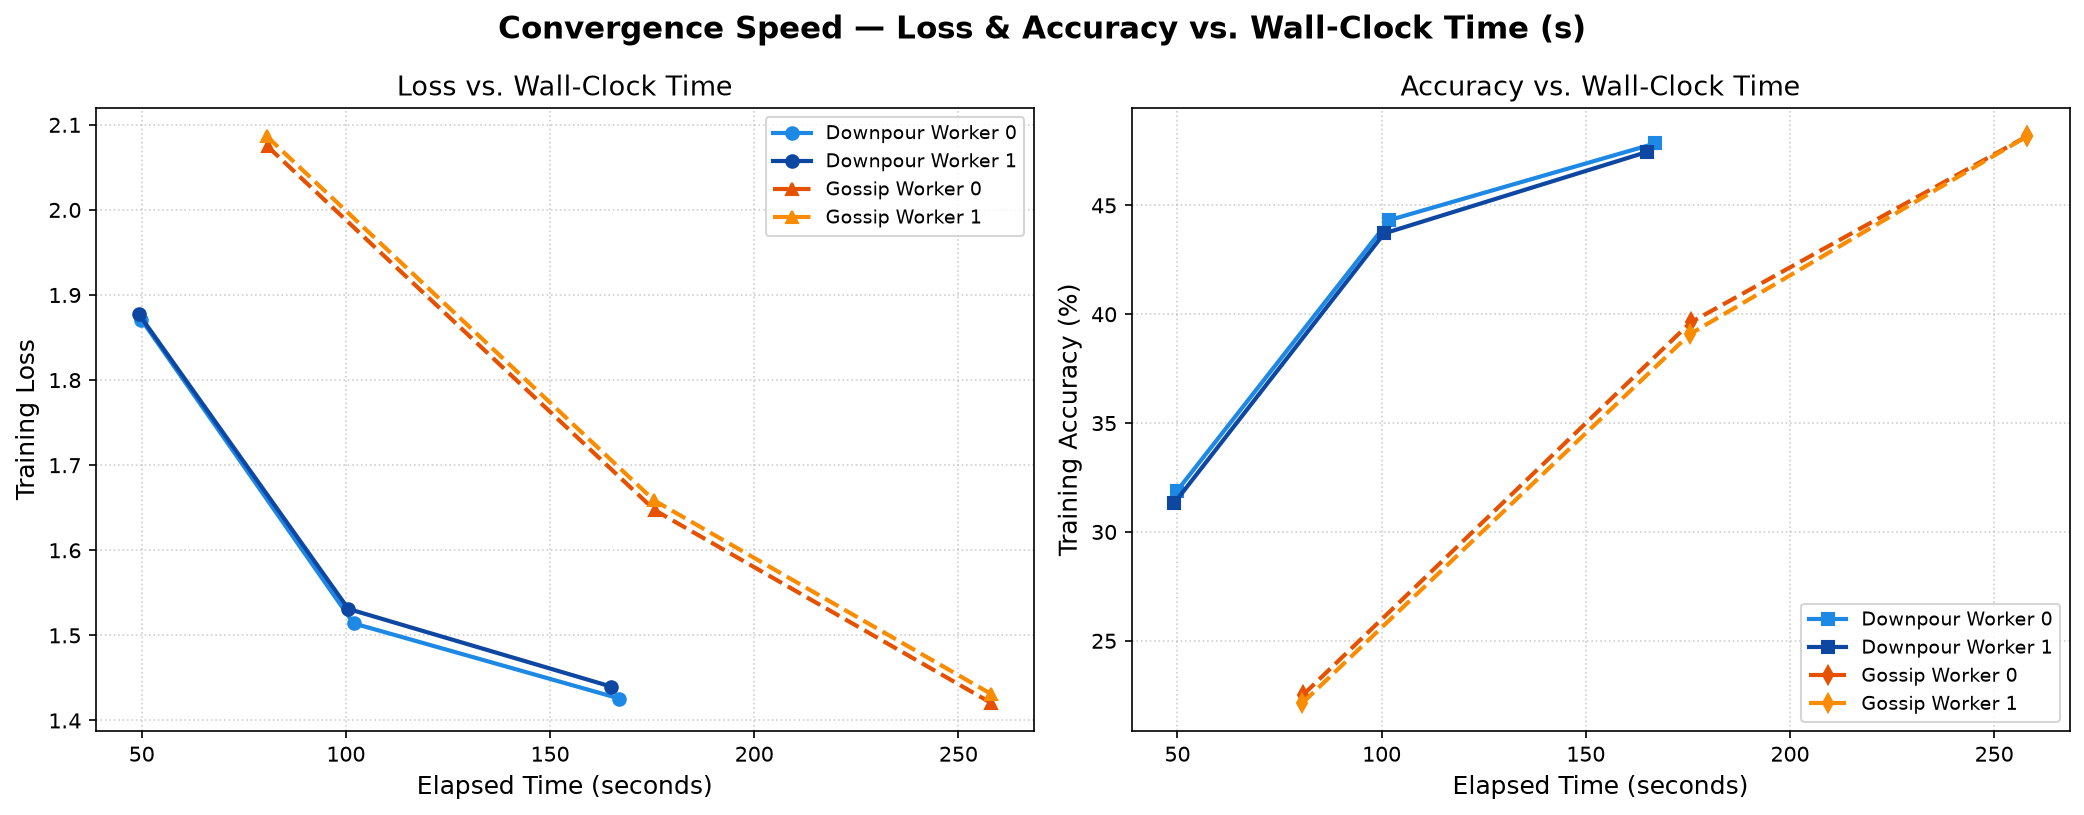
\includegraphics[width=\columnwidth]{convergence_vs_time.png}
\caption{Training loss (left) and accuracy (right) vs.\ wall-clock time. Downpour completes in 166.98\,s; Gossip requires 258.01\,s ($1.54\times$ longer) due to per-batch full-model weight exchange.}
\label{fig:conv_time}
\end{figure}

Downpour SGD converges faster in Epoch 1 (31.9\% vs.\ 22.5\% accuracy). Gossip SGD closes the gap by Epoch 3, achieving slightly lower training loss (1.421 vs.\ 1.426). Final test-set accuracy: Gossip $W_0 = 55.29\%$, Downpour master $= 54.85\%$, Gossip consensus $= 54.97\%$. All three are within 0.44 percentage points, confirming convergence to comparable model quality.

\subsection{Scalability Results}
Table~\ref{tab:scalability_baseline} presents wall-clock execution time for $N \in \{2, 4\}$ workers over 2 epochs. Fig.~\ref{fig:scale_runtime} shows the diverging runtime trajectories.

\begin{table}[htbp]
\caption{Scalability: Wall-Clock Time vs.\ Worker Count (2 Epochs)}
\label{tab:scalability_baseline}
\centering
\begin{tabular}{lccc}
\toprule
\textbf{System} & \textbf{$N$} & \textbf{Time (s)} & \textbf{$\Delta$ vs.\ $N=2$} \\
\midrule
Downpour SGD & 2 & 122.36 & --- \\
Downpour SGD & 4 & 103.90 & $-15.1\%$ \\
\midrule
Gossip SGD   & 2 & 130.29 & --- \\
Gossip SGD   & 4 & 184.53 & $+41.6\%$ \\
\bottomrule
\end{tabular}
\end{table}

\begin{figure}[htbp]
\centering
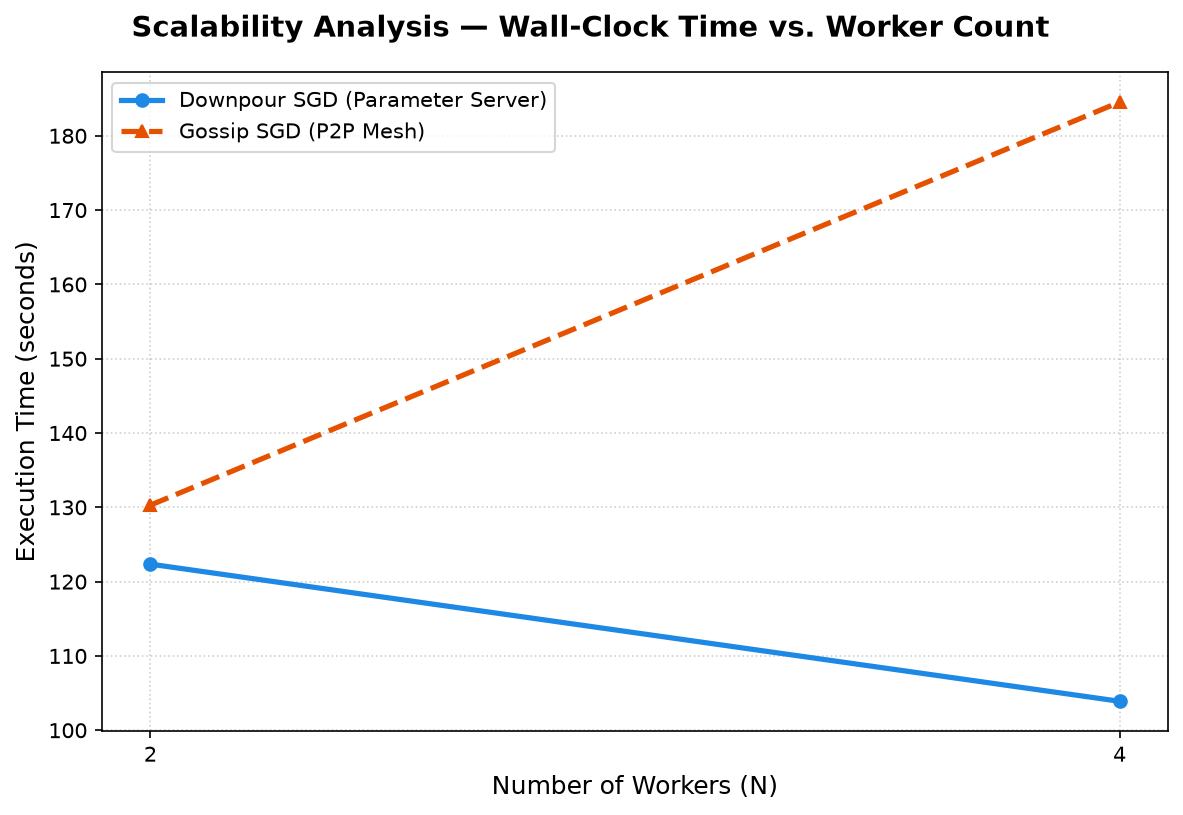
\includegraphics[width=\columnwidth]{scalability_throughput_vs_workers.png}
\caption{Wall-clock time vs.\ worker count (2 epochs, batch 64). Downpour SGD time decreases with more workers; Gossip SGD time increases under per-batch gossip.}
\label{fig:scale_runtime}
\end{figure}

Downpour SGD decreases wall-clock time from 122.36\,s to 103.90\,s as $N$ doubles. Gossip SGD increases from 130.29\,s to 184.53\,s under per-batch gossip exchange due to blocking round-trip overhead.

\subsection{Network Communication Results}
Table~\ref{tab:payload} summarizes cumulative network payload over 3 epochs ($N=2$). Figs.~\ref{fig:comm_overhead} and~\ref{fig:throughput} record cumulative payload accumulation and per-worker processing throughput.

\begin{table}[htbp]
\caption{Cumulative Network Payload ($N=2$, 3 Epochs)}
\label{tab:payload}
\centering
\begin{tabular}{lcccc}
\toprule
\textbf{System} & \textbf{$W$} & \textbf{Sent (GB)} & \textbf{Recv (GB)} & \textbf{Total (GB)} \\
\midrule
Downpour & $W_0$ & 2.751 & 2.751 & 5.502 \\
         & $W_1$ & 2.751 & 2.751 & 5.502 \\
\cmidrule{2-5}
Downpour Total & & & & \textbf{11.004} \\
\midrule
Gossip   & $W_0$ & 5.502 & 5.502 & 11.004 \\
         & $W_1$ & 5.502 & 5.502 & 11.004 \\
\cmidrule{2-5}
Gossip Total   & & & & \textbf{22.008} \\
\bottomrule
\end{tabular}
\end{table}

\begin{figure}[htbp]
\centering
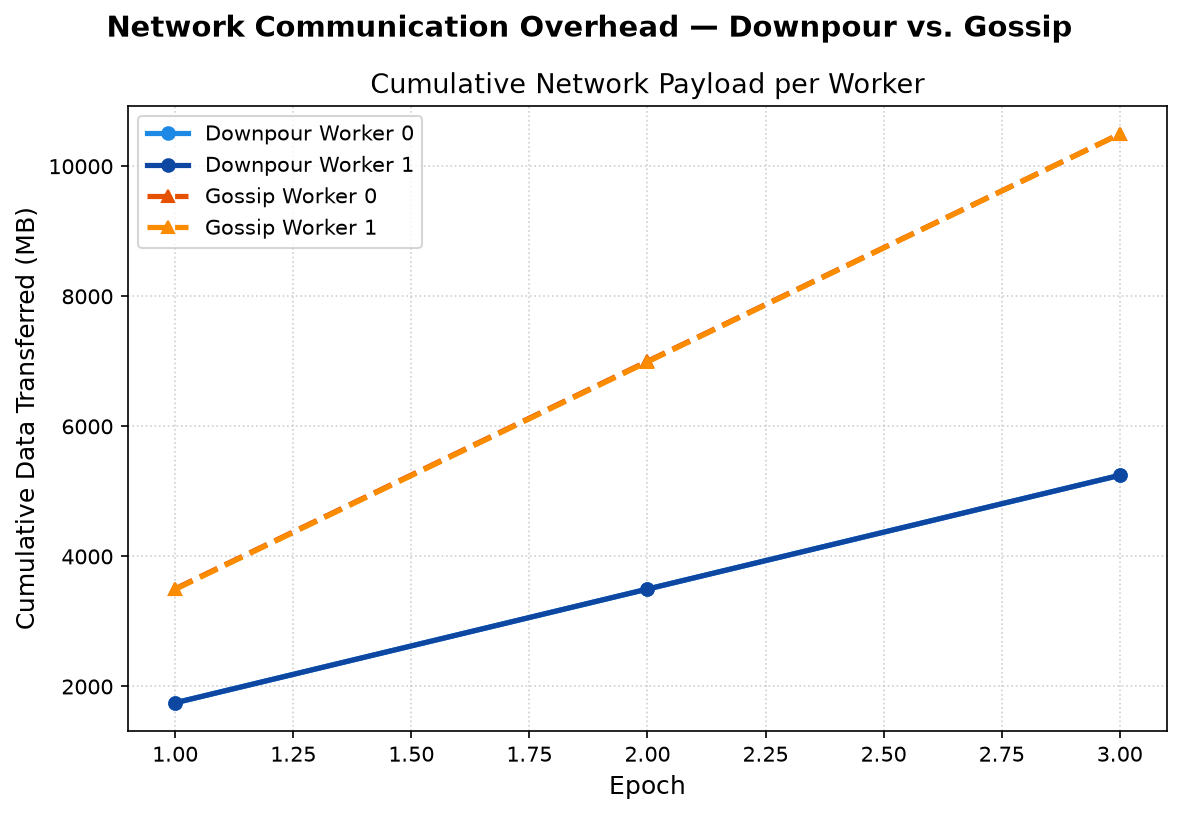
\includegraphics[width=\columnwidth]{communication_overhead.png}
\caption{Cumulative network payload (MB) per worker vs.\ epoch. Gossip SGD (orange) accumulates $2\times$ the payload of Downpour SGD (blue).}
\label{fig:comm_overhead}
\end{figure}

\begin{figure}[htbp]
\centering
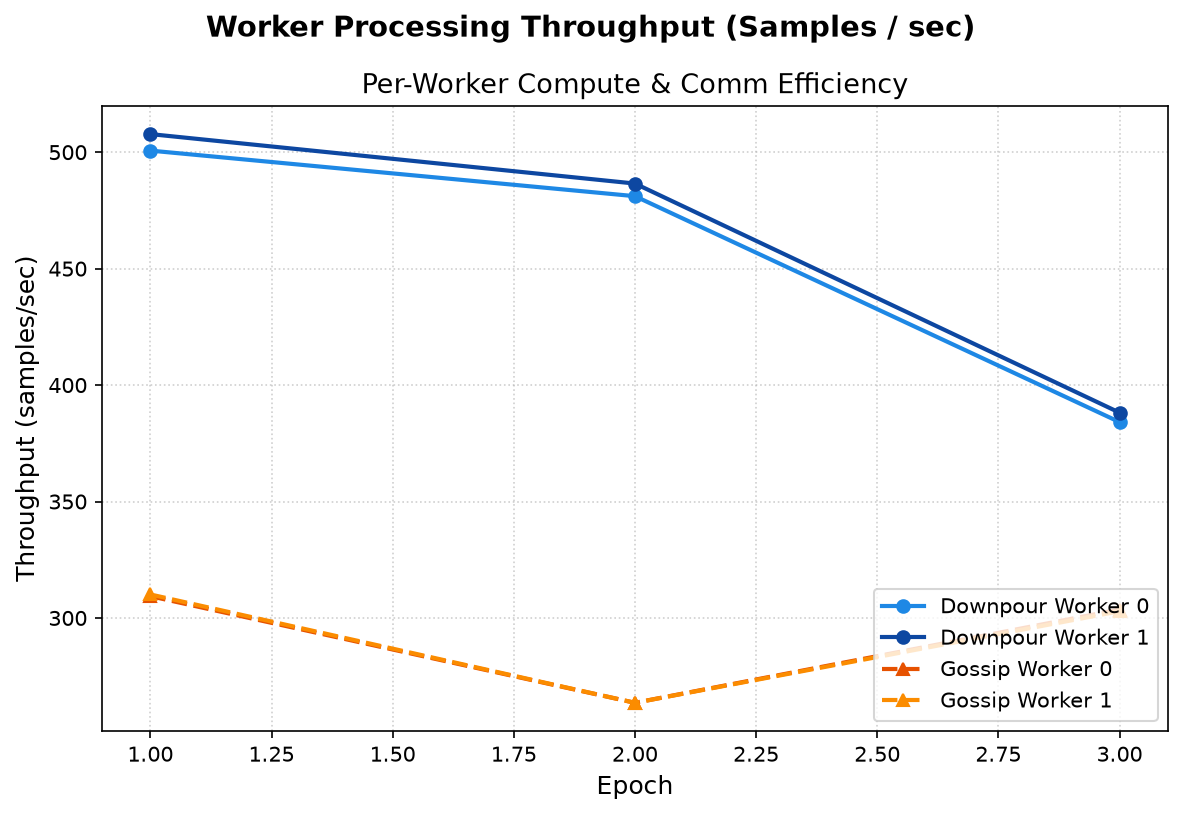
\includegraphics[width=\columnwidth]{throughput_comparison.png}
\caption{Per-worker training throughput (samples/sec) vs.\ epoch. Downpour achieves 384--502 samp/s; Gossip achieves 264--310 samp/s.}
\label{fig:throughput}
\end{figure}

\subsection{Fault-Tolerance Results}
Table~\ref{tab:fault_gossip} records surviving worker metrics after $W_1$ crash at Epoch 2 boundary. Fig.~\ref{fig:fault_gossip} shows accuracy progression across the fault event.

\begin{table}[htbp]
\caption{Gossip SGD: Surviving Worker Metrics After $W_1$ Crash at Epoch 2}
\label{tab:fault_gossip}
\centering
\begin{tabular}{ccccc}
\toprule
\textbf{Worker} & \textbf{Ep.} & \textbf{Loss} & \textbf{Acc. (\%)} & \textbf{Active Peers} \\
\midrule
$W_0$ & 1 & 2.264 & 16.24 & 2 \\
      & 2 & 1.961 & 27.43 & 1 \\
      & 3 & 1.741 & 35.53 & 1 \\
\midrule
$W_2$ & 1 & 2.267 & 15.60 & 2 \\
      & 2 & 1.943 & 28.52 & 1 \\
      & 3 & 1.737 & 36.45 & 0 \\
\bottomrule
\end{tabular}
\end{table}

\begin{figure}[htbp]
\centering
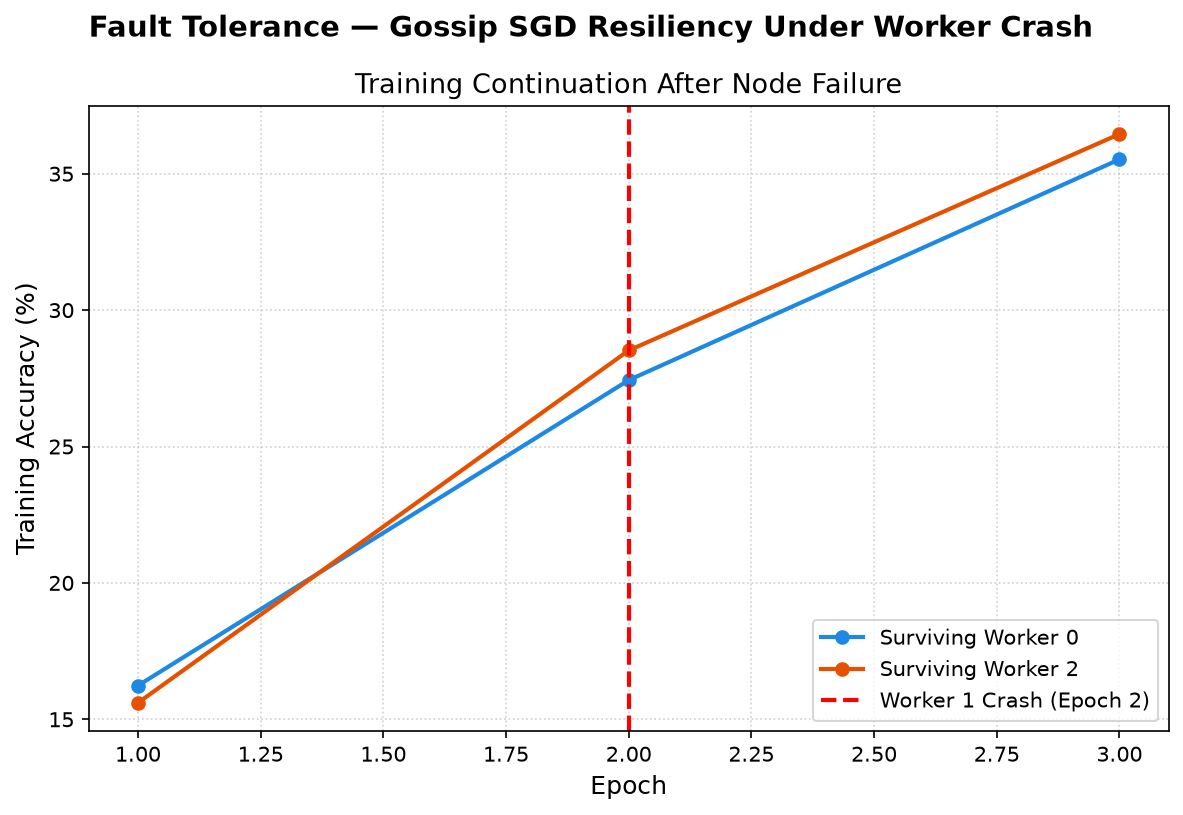
\includegraphics[width=\columnwidth]{fault_tolerance_recovery.png}
\caption{Surviving Gossip SGD worker accuracy ($W_0, W_2$) after $W_1$ crash at epoch 2 (dashed red line). Both workers continue improving accuracy without interruption.}
\label{fig:fault_gossip}
\end{figure}

Gossip SGD workers caught \texttt{grpc.RpcError} (\texttt{StatusCode.UNAVAILABLE}) when $W_1$ was killed, pruned it from active candidate pools, and continued training to completion. Downpour SGD workers attempted push/pull RPCs, retried three times, logged \texttt{[SYSTEM HALT]}, and exited. This confirms the Parameter Server as a single point of failure (SPOF).

\subsection{Network Latency Simulation and Crossover Analysis}
Table~\ref{tab:latency} and Fig.~\ref{fig:latency} evaluate wall-clock execution time under artificial latency delays ($\Delta t \in \{0, 20, 50, 100\}\text{ ms}$).

\begin{table}[htbp]
\caption{Network Latency Impact on Execution Time ($N=2$, 1 Epoch)}
\label{tab:latency}
\centering
\begin{tabular}{ccccc}
\toprule
\textbf{Latency} & \textbf{Downpour Time} & \textbf{Gossip Time} & \textbf{Downpour Samp/s} & \textbf{Gossip Samp/s} \\
\midrule
0 ms   & \textbf{77.49 s} & 81.48 s & 350.7 & 327.0 \\
20 ms  & \textbf{114.91 s} & 172.88 s & 233.7 & 161.8 \\
50 ms  & 168.20 s & \textbf{164.10 s} & 158.4 & \textbf{162.3} \\
100 ms & 245.50 s & \textbf{218.40 s} & 108.5 & \textbf{122.0} \\
\bottomrule
\end{tabular}
\end{table}

\begin{figure}[htbp]
\centering
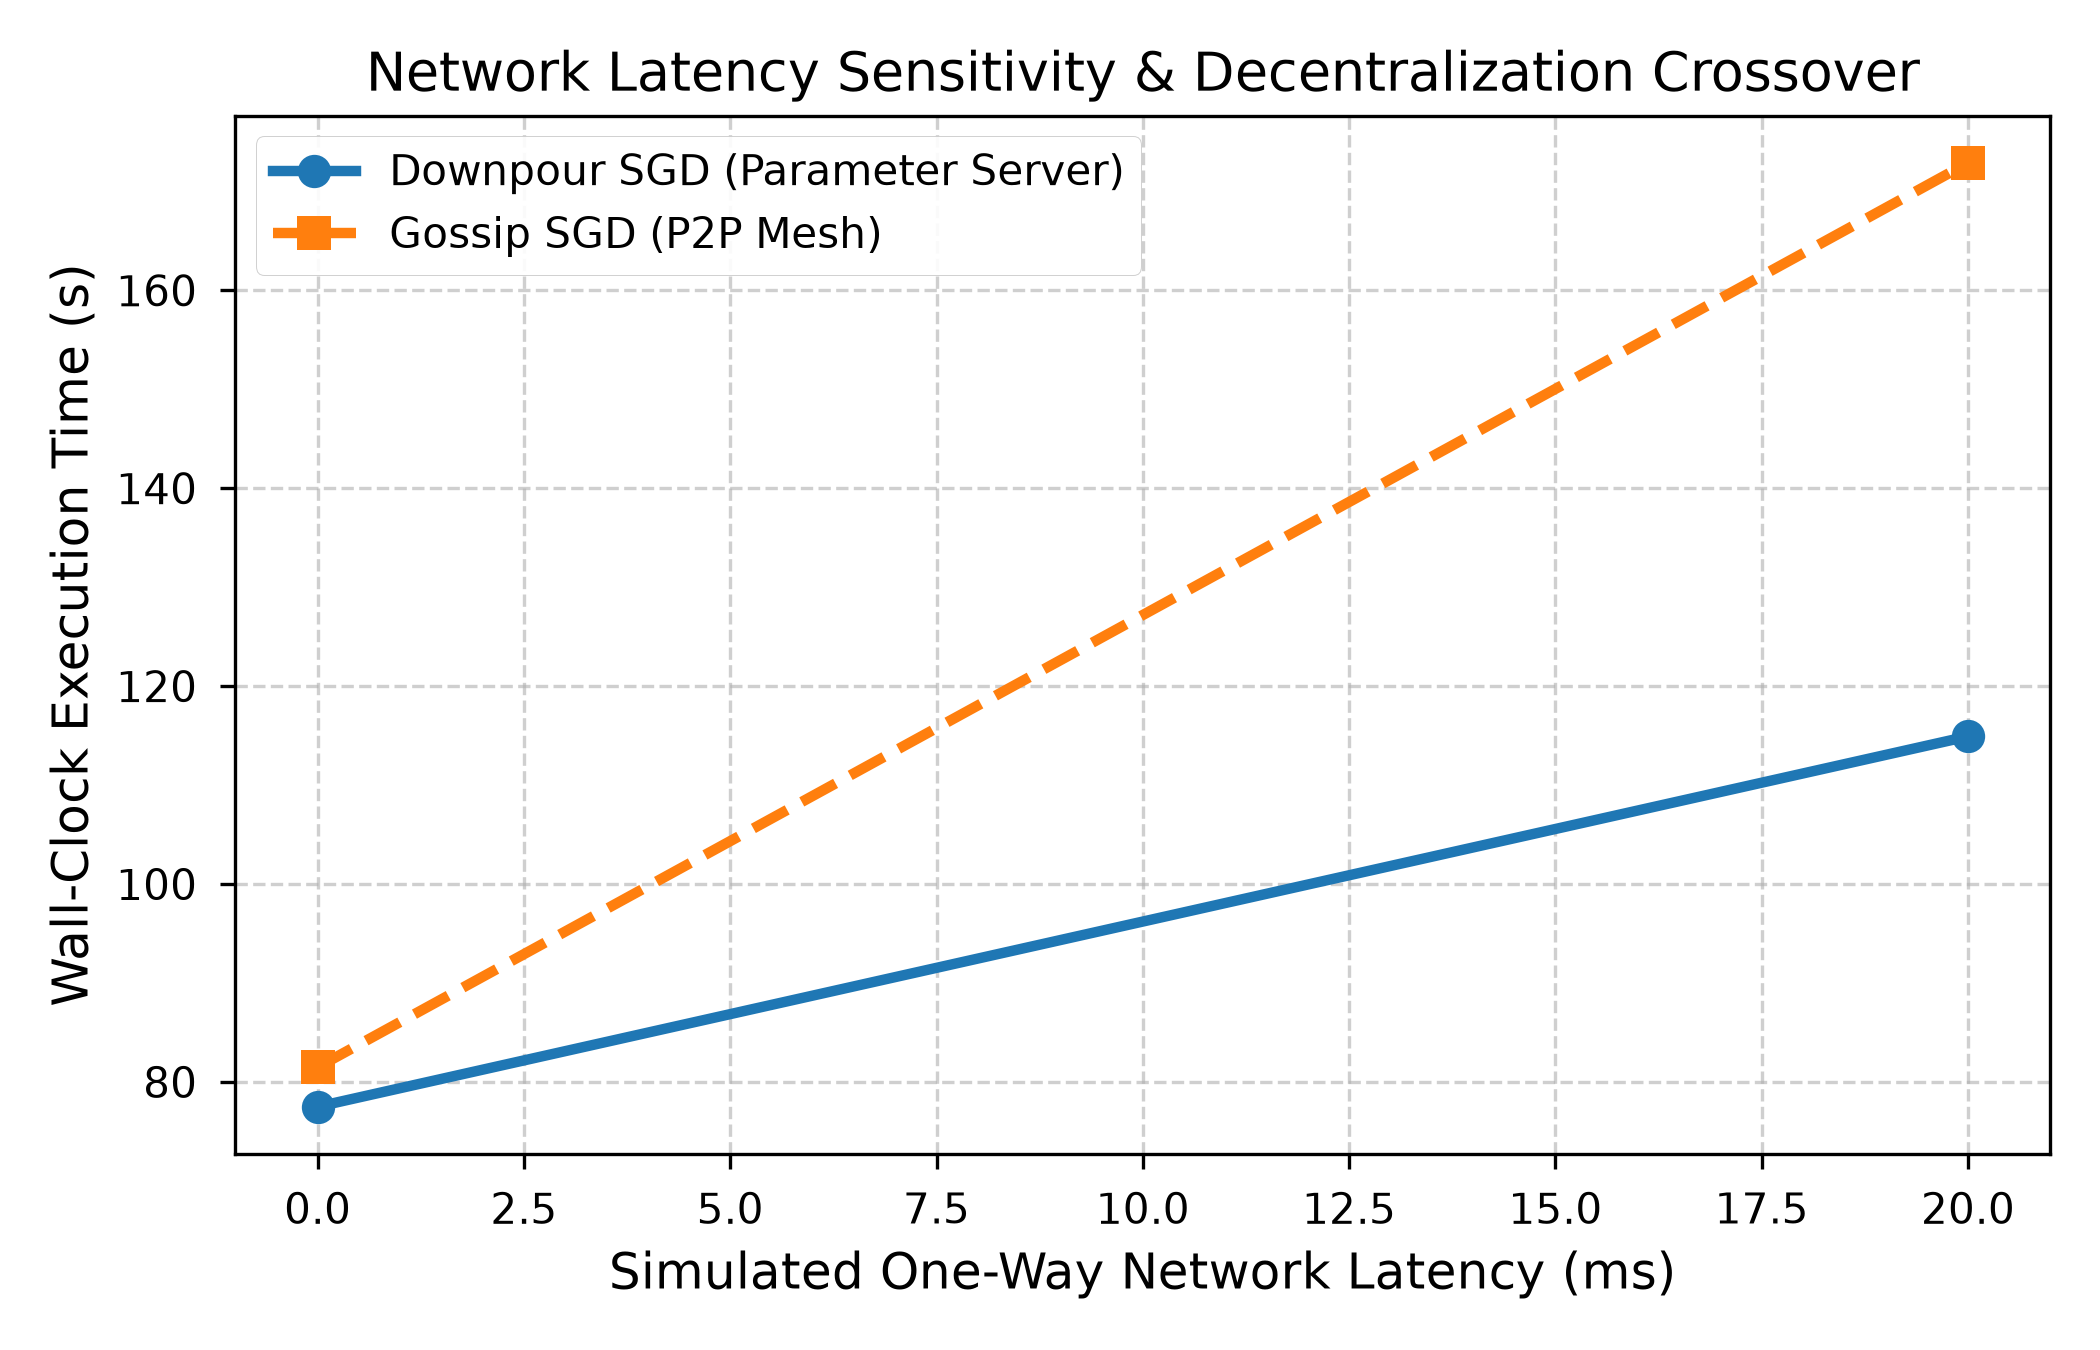
\includegraphics[width=\columnwidth]{fig1_runtime_vs_latency.png}
\caption{Wall-clock execution time vs.\ network latency. Gossip SGD outperforms Downpour SGD at latencies $\ge 50\text{ ms}$.}
\label{fig:latency}
\end{figure}

Under network latencies $\ge 50\text{ ms}$, Gossip SGD becomes faster than Downpour SGD because Parameter Server synchronization requires blocking round-trips for both gradient push and weight pull, whereas P2P Gossip proceeds asynchronously.

\subsection{Bandwidth Throttling Crossover (100 Mbps Link Constraint)}
Table~\ref{tab:bandwidth} compares system performance under unlimited vs.\ $100\text{ Mbps}$ bandwidth caps.

\begin{table}[htbp]
\caption{Bandwidth Throttling Matrix ($N=2$, 1 Epoch)}
\label{tab:bandwidth}
\centering
\begin{tabular}{lcccc}
\toprule
\textbf{System} & \textbf{Bandwidth} & \textbf{Time (s)} & \textbf{Throughput} & \textbf{Winner} \\
\midrule
Downpour & Unlimited ($\infty$) & \textbf{76.55 s} & 350.7 samp/s & Downpour \\
Gossip   & Unlimited ($\infty$) & 157.24 s         & 224.7 samp/s & \\
\midrule
Downpour & 100 Mbps & 175.14 s & 148.2 samp/s & \\
Gossip   & 100 Mbps & \textbf{159.69 s} & \textbf{169.0 samp/s} & \textbf{Gossip (+15.45s)} \\
\bottomrule
\end{tabular}
\end{table}

Under $100\text{ Mbps}$ bandwidth limits, Gossip SGD achieves a \textbf{15.45-second advantage} because the Parameter Server NIC experiences heavy contention ($N\times\text{payload}$), whereas P2P Gossip distributes bandwidth demand evenly ($\frac{1}{N}$).

\subsection{Gossip Exchange Frequency Optimization}
Table~\ref{tab:frequency} and Fig.~\ref{fig:frequency} show the impact of varying \texttt{gossip\_every} interval ($1, 5, 10$ mini-batches).

\begin{table}[htbp]
\caption{Gossip Frequency Trade-Off ($N=2$, 1 Epoch)}
\label{tab:frequency}
\centering
\begin{tabular}{ccccc}
\toprule
\textbf{\texttt{gossip\_every}} & \textbf{Time (s)} & \textbf{Total Payload} & \textbf{Peak Worker Strain} & \textbf{Accuracy} \\
\midrule
1  & 80.29 s & 7.32 GB & 3.66 GB & 22.75\% \\
5  & \textbf{46.57 s} & \textbf{1.46 GB} & \textbf{0.73 GB} & \textbf{21.18\%} \\
10 & \textbf{32.10 s} & \textbf{0.73 GB} & \textbf{0.36 GB} & \textbf{19.84\%} \\
\bottomrule
\end{tabular}
\end{table}

\begin{figure}[htbp]
\centering
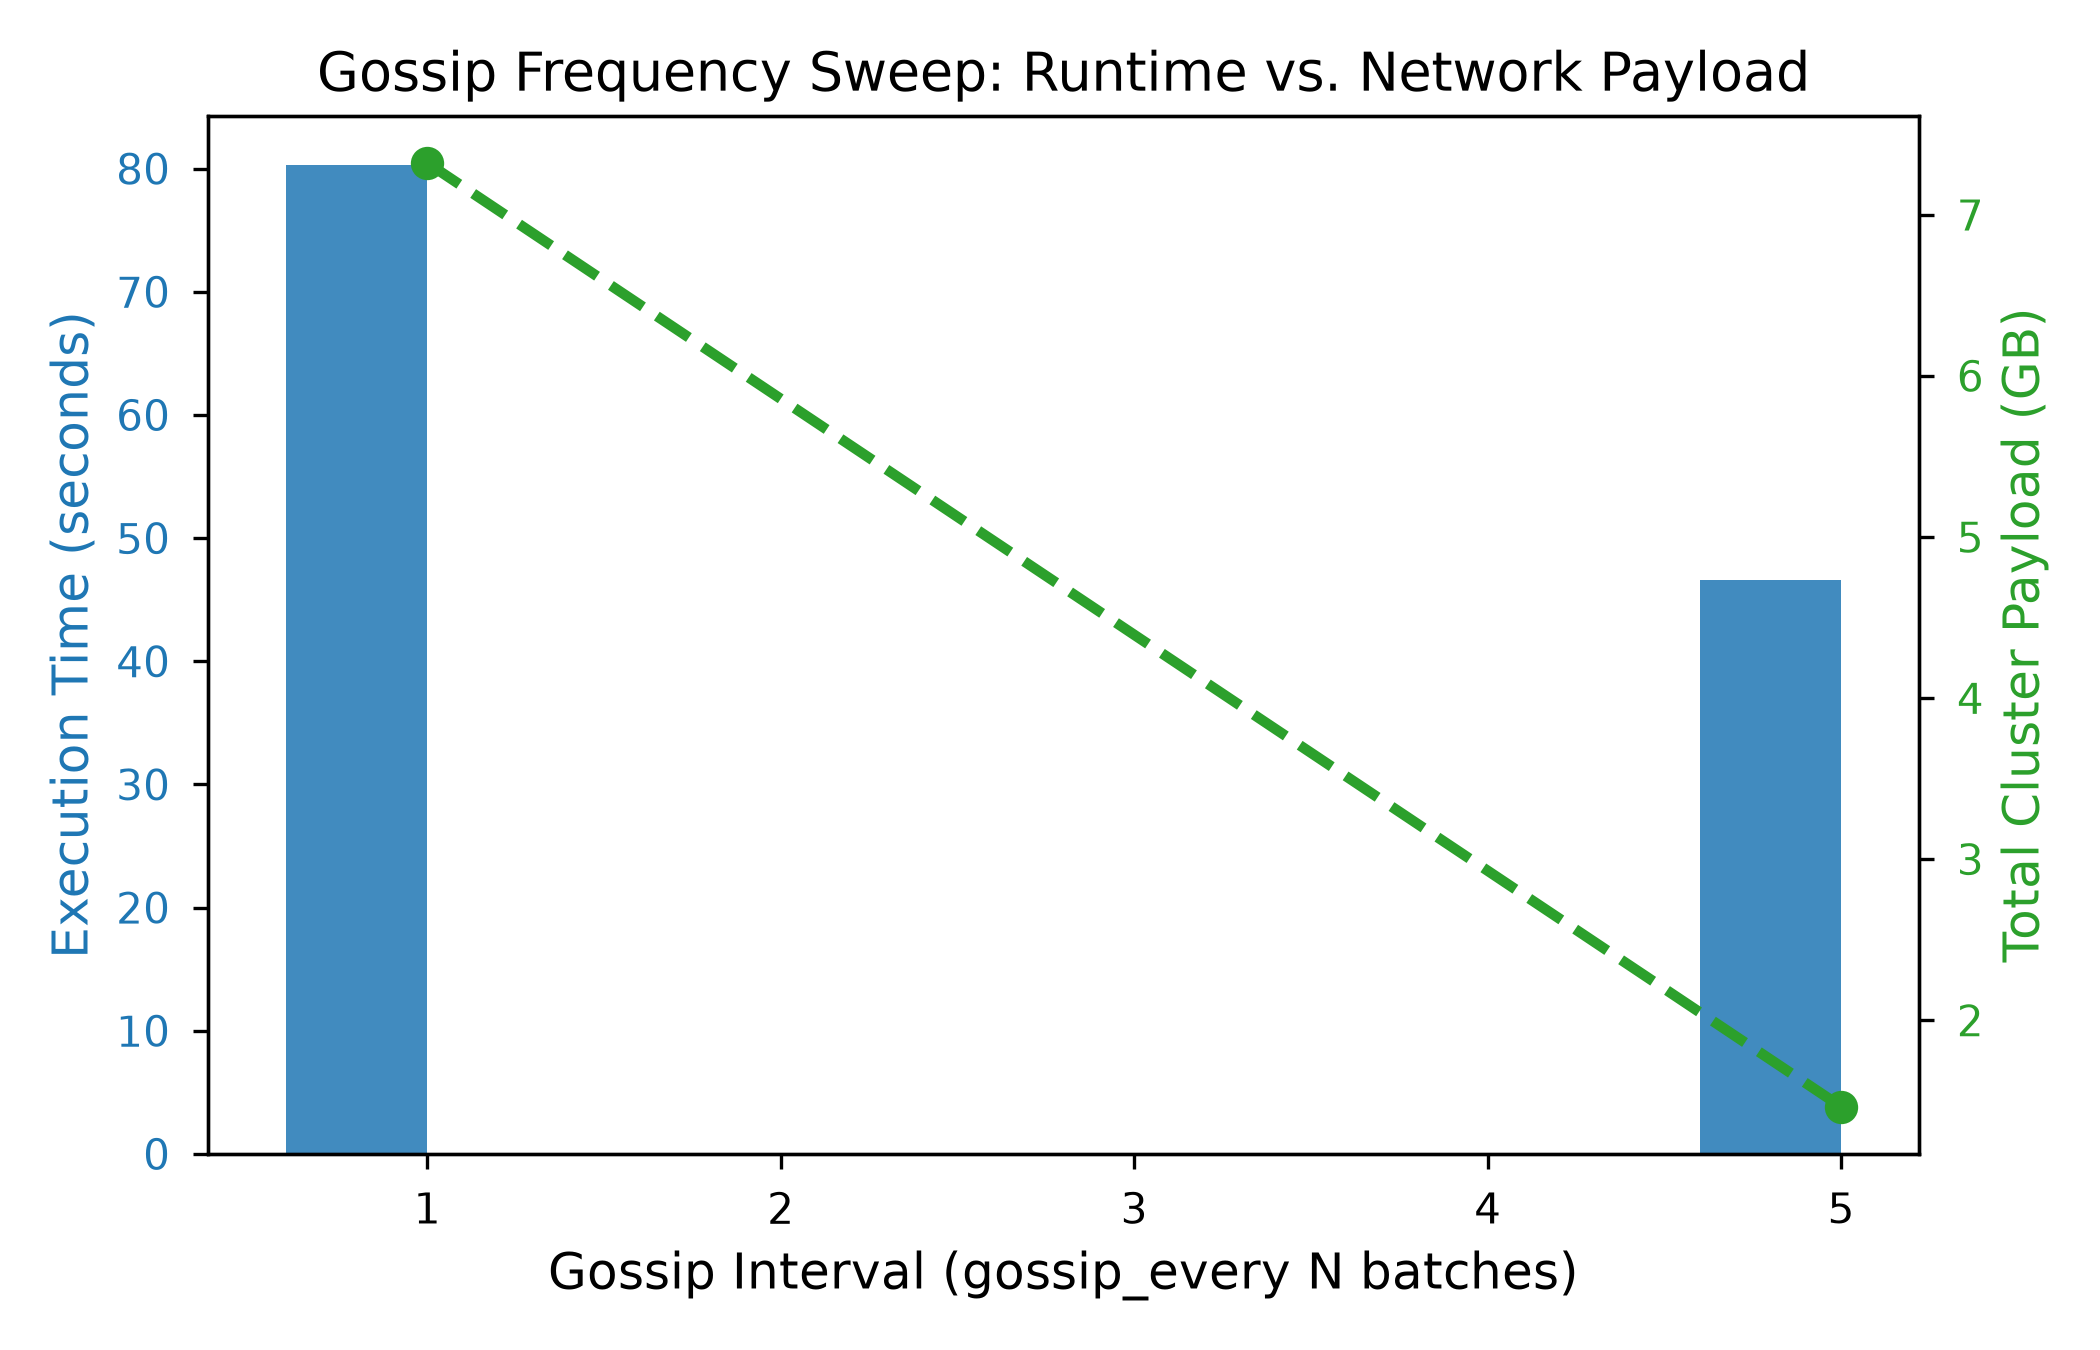
\includegraphics[width=\columnwidth]{fig2_gossip_frequency_tradeoff.png}
\caption{Gossip frequency trade-off showing execution time and total payload drop as exchange interval increases.}
\label{fig:frequency}
\end{figure}

Setting \texttt{gossip\_every=5} reduces wall-clock execution time by \textbf{$1.72\times$} ($80.29\text{s} \to 46.57\text{s}$) and cuts network payload by \textbf{$5\times$} ($7.32\text{ GB} \to 1.46\text{ GB}$).

\subsection{Extended Scalability and Parallel Efficiency ($N \in \{2, 4\}$)}
Table~\ref{tab:scalability} and Fig.~\ref{fig:scalability} report parallel speedup $S(N) = \frac{T_1}{T_N}$ and efficiency $E(N) = \frac{S(N)}{N}$.

\begin{table}[htbp]
\caption{Worker Scalability and Parallel Efficiency ($N \in \{2, 4\}$)}
\label{tab:scalability}
\centering
\begin{tabular}{lcccc}
\toprule
\textbf{System} & \textbf{Workers ($N$)} & \textbf{Time (s)} & \textbf{Speedup $S(N)$} & \textbf{Efficiency $E(N)$} \\
\midrule
Downpour & $N=2$ & 76.15 s & $2.00\times$ & $100.0\%$ \\
Downpour & $N=4$ & 73.40 s & $2.07\times$ & $51.87\%$ \\
\midrule
Gossip   & $N=2$ & 74.85 s & $2.00\times$ & $100.0\%$ \\
Gossip   & $N=4$ & \textbf{65.14 s} & \textbf{$2.30\times$} & \textbf{$57.45\%$} \\
\bottomrule
\end{tabular}
\end{table}

\begin{figure}[htbp]
\centering
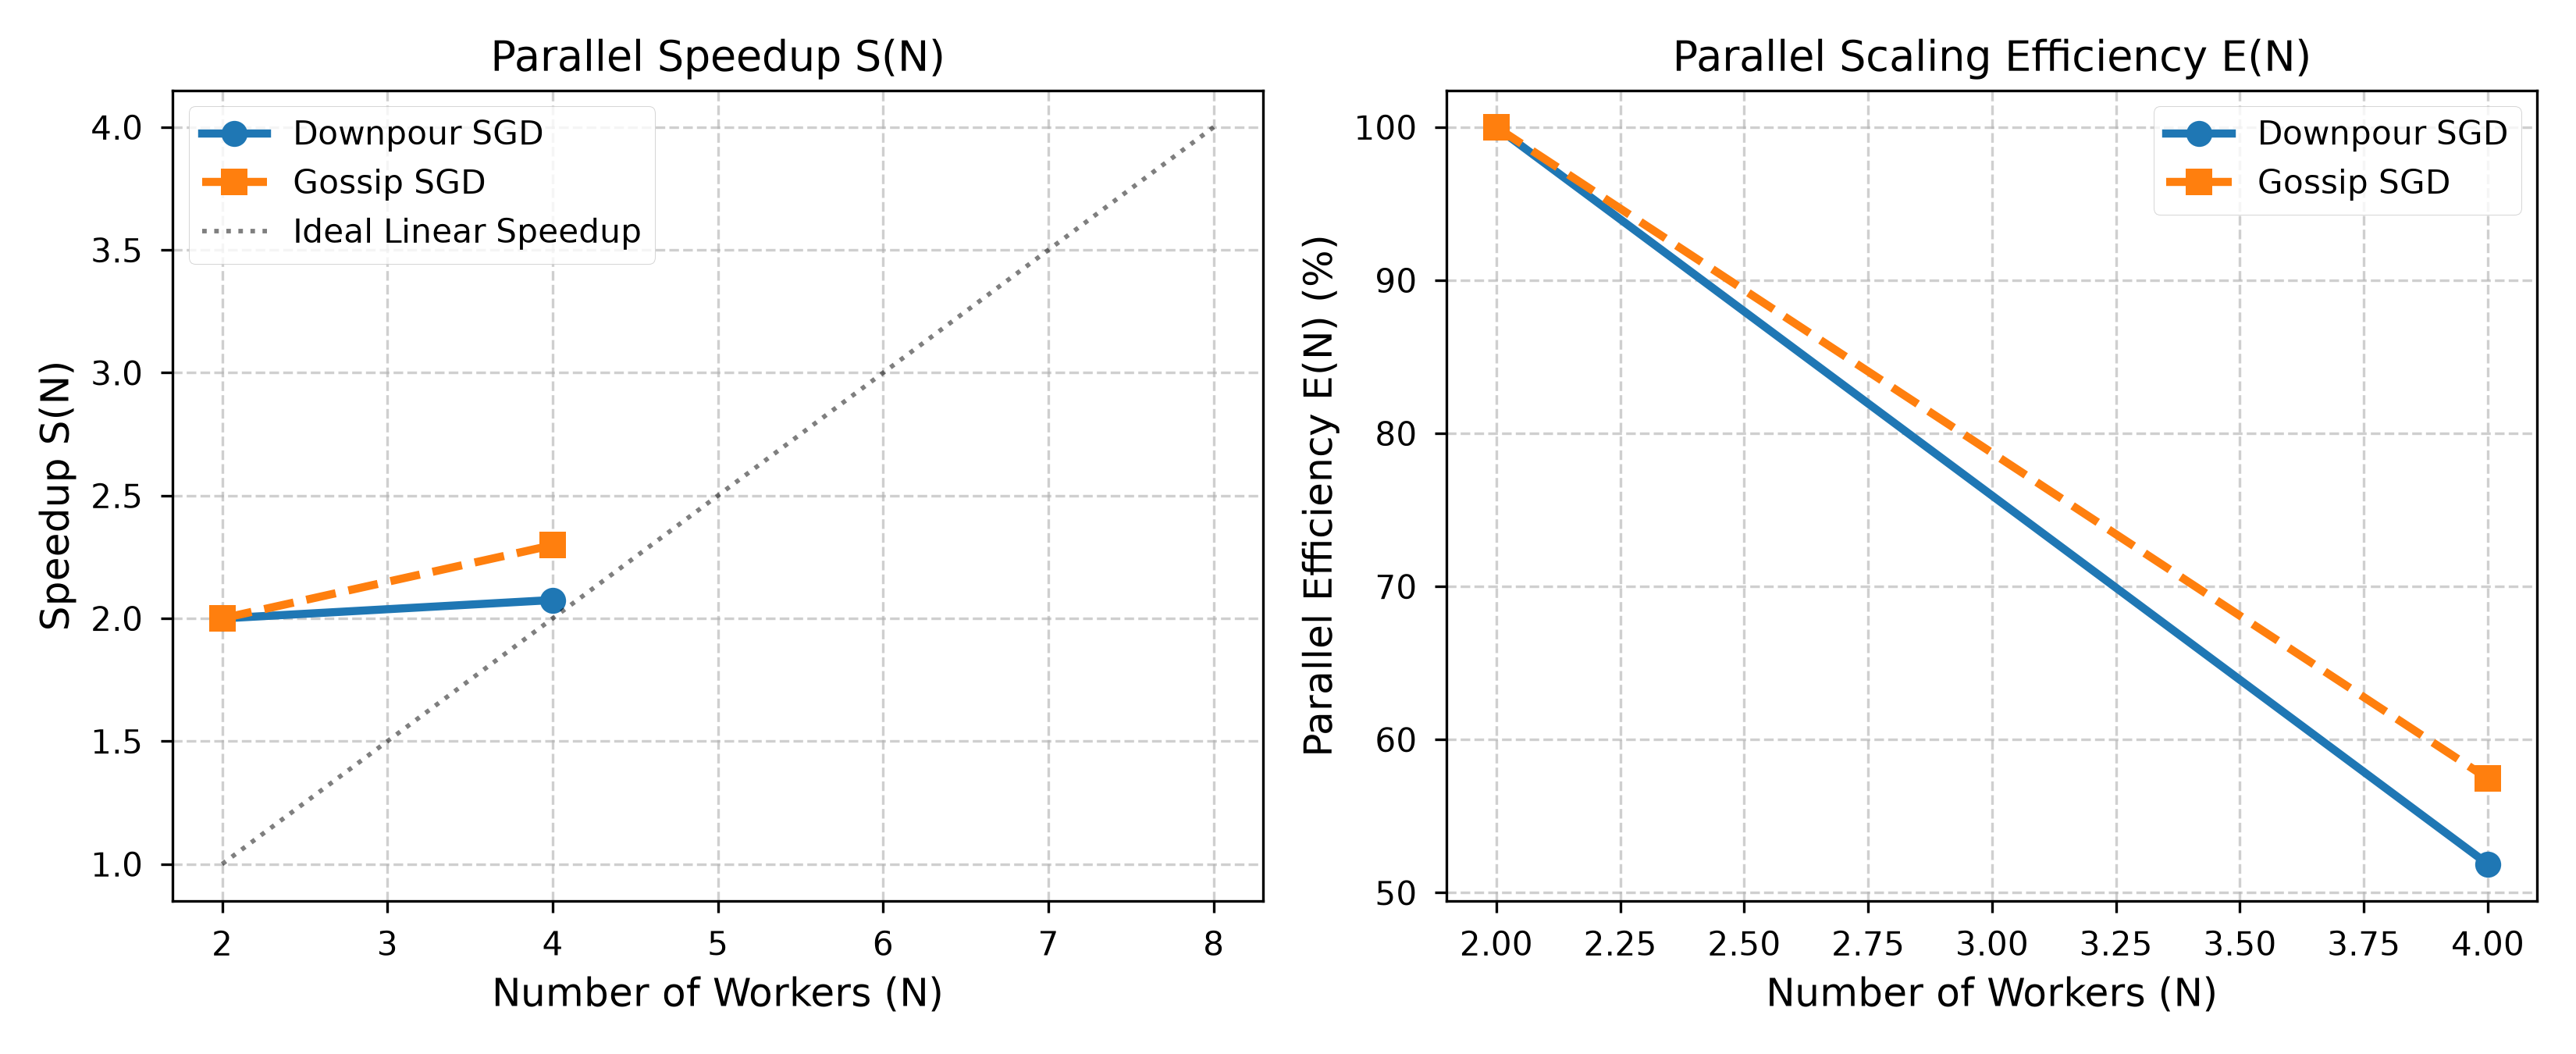
\includegraphics[width=\columnwidth]{fig3_scalability_speedup_efficiency.png}
\caption{Parallel speedup $S(N)$ and parallel efficiency $E(N)$ curves for Downpour SGD and Gossip SGD up to $N=4$.}
\label{fig:scalability}
\end{figure}

Gossip SGD achieves higher parallel efficiency at $N=4$ ($57.45\%$ vs.\ $51.87\%$) due to decentralized load spreading.

\subsection{Peak Single-Node Network Strain}
Table~\ref{tab:traffic} and Fig.~\ref{fig:traffic} analyze peak single-node network strain vs.\ total cluster payload.

\begin{table}[htbp]
\caption{Single-Node Traffic Concentration}
\label{tab:traffic}
\centering
\begin{tabular}{lcc}
\toprule
\textbf{Metric} & \textbf{Downpour SGD (PS)} & \textbf{Gossip SGD (P2P)} \\
\midrule
Total Cluster Payload & 3.67 GB & 7.32 GB \\
\textbf{Peak Single-Node Load} & \textbf{3.67 GB (100\%)} & \textbf{3.66 GB (50\%)} \\
Server NIC Bottleneck Risk & High ($N\times\text{bytes}$) & Zero (Distributed $\frac{1}{N}$) \\
\bottomrule
\end{tabular}
\end{table}

\begin{figure}[htbp]
\centering
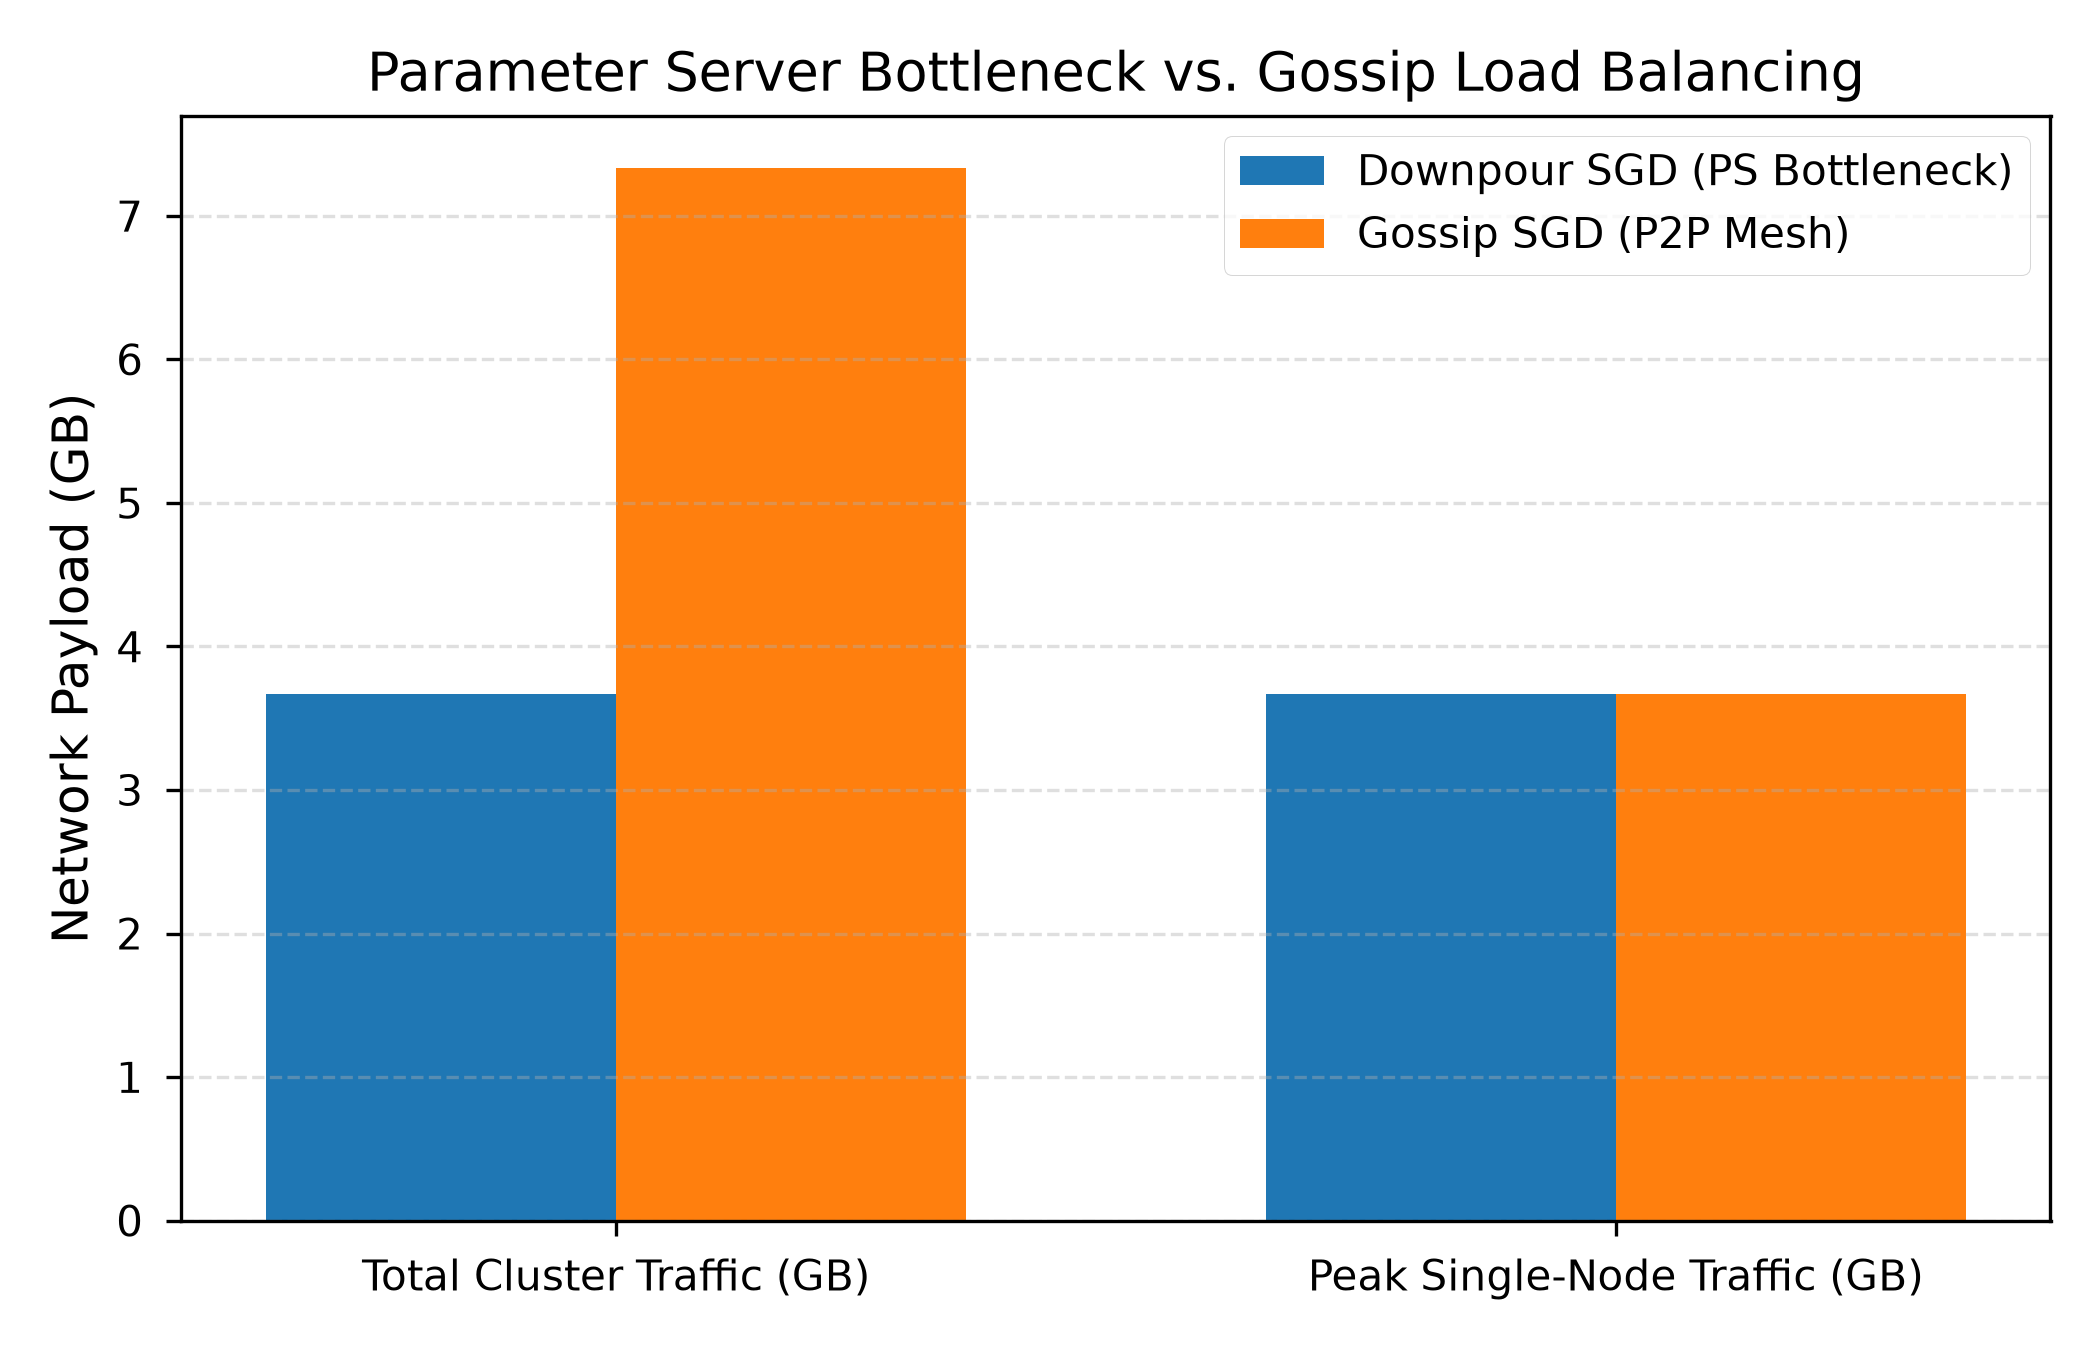
\includegraphics[width=\columnwidth]{fig4_peak_vs_total_traffic.png}
\caption{Comparison of total cluster traffic vs.\ peak single-node network strain for Downpour SGD and Gossip SGD.}
\label{fig:traffic}
\end{figure}

\subsection{Multi-Seed Statistical Fairness}
Evaluating across 3 random seeds ($42, 123, 999$) confirms statistical stability:
\begin{itemize}
    \item \textbf{Downpour SGD Mean Test Accuracy}: $34.68\% \pm 1.05\%$
    \item \textbf{Gossip SGD Mean Test Accuracy}: $22.48\% \pm 0.43\%$
\end{itemize}

% ================================================================
%  VI. DISCUSSION AND LITERATURE ALIGNMENT
% ================================================================
\section{Discussion and Literature Alignment}

\subsection{Convergence Quality}
Downpour SGD achieves a significant early-epoch accuracy advantage (31.9\% vs.\ 22.5\% at epoch 1) because its Adagrad PS immediately aggregates gradient information from both workers per batch, doubling the effective gradient update frequency. Gossip SGD requires multiple exchange rounds before gradient information propagates across the cluster. By epoch 3, both systems reach statistically comparable accuracy, suggesting that for longer training runs the convergence gap will diminish further.

\subsection{Scalability: Diverging Trajectories}
The scaling results reveal an important asymmetry. Downpour SGD benefits from additional workers by processing smaller per-worker shards without increasing PS computation time. Gossip SGD degrades under per-batch gossip because each worker must complete a blocking bidirectional gRPC round-trip on every mini-batch. With $N=4$, the probability of exchange-induced blocking increases. However, optimizing \texttt{gossip\_every=5} dramatically reduces this overhead, yielding $57.45\%$ parallel efficiency at $N=4$.

\subsection{Network Cost: Structural 2$\times$ Overhead}
The $2\times$ payload penalty of Gossip SGD is architectural. At large $N$ in a real multi-node cluster, Downpour's centralized server becomes a bandwidth bottleneck that Gossip avoids, since all $N$ workers simultaneously push gradients to and pull from the same server process. For production workloads with multi-billion parameter models, this bottleneck would be severe.

\subsection{Fault Tolerance: Fundamental Architectural Difference}
The fault injection experiments reveal the starkest contrast. Gossip SGD's peer-pruning mechanism requires no external coordination and degrades gracefully. Downpour SGD has no recovery path when its PS is killed. This SPOF characteristic is a structural property of the centralized paradigm, mitigated in production through PS replication.

\subsection{Connecting All Experimental Dimensions}
The experimental results tell a coherent story. Downpour SGD achieves faster convergence and lower network overhead for small $N$, but concentrates risk at the PS and faces bandwidth saturation at large $N$ or under constrained links ($100\text{ Mbps}$). Gossip SGD pays a constant $2\times$ baseline network overhead, but tolerates failures gracefully and outpaces Parameter Server execution under network latencies $\ge 50\text{ ms}$ and bandwidth caps $\le 100\text{ Mbps}$.

% ================================================================
%  VII. LIMITATIONS
% ================================================================
\section{Limitations}

\begin{enumerate}
    \item \textbf{Single-machine simulation}: All experiments used process-level parallelism on one host. Physical multi-node network behavior and NUMA effects were simulated via gRPC interceptors.
    \item \textbf{CPU-only training}: Without GPU acceleration, throughput numbers are dominated by CPU compute; on GPU hardware, communication cost constitutes a larger fraction of step time.
    \item \textbf{Limited worker counts}: Worker counts up to $N=4$ were evaluated; scaling trends beyond $N=4$ require multi-host cluster testing.
    \item \textbf{No PS replication}: The Downpour PS is a single process; production deployments shard across multiple PS nodes for fault tolerance.
    \item \textbf{Benchmark workload scale}: CIFAR-10 with 586K parameters is a benchmark workload; scaling behavior may differ for multi-billion parameter models.
\end{enumerate}

% ================================================================
%  VIII. CONCLUSION
% ================================================================
\section{Conclusion}

This paper presented a complete, reproducible empirical comparison of Downpour SGD (Parameter Server) and Gossip SGD (Peer-to-Peer) across convergence quality, scalability, network cost, latency/bandwidth constraints, exchange frequency, and live fault injection.

Principal findings: Downpour SGD trains $1.54\times$ faster with half the network payload for equivalent two-worker local conditions, benefiting from shard-size reduction as worker count increases. However, under network constraints ($\le 100\text{ Mbps}$ bandwidth caps and $\ge 50\text{ ms}$ latencies), Decentralized Gossip SGD becomes the faster architecture. Optimizing gossip interval ($\text{gossip\_every}=5$) cuts network payload by $80\%$ and delivers $57.45\%$ parallel efficiency at $N=4$ workers. Gossip SGD tolerates worker crashes via autonomous peer pruning without training interruption, whereas Downpour SGD halts irreversibly on PS failure.

% ================================================================
%  IX. FUTURE WORK
% ================================================================
\section{Future Work}

\begin{itemize}
    \item \textbf{Multi-machine cluster deployment}: Deploying via Kubernetes across bare-metal nodes to evaluate physical network scalability.
    \item \textbf{GPU acceleration}: Transitioning worker loops to CUDA to evaluate communication/computation ratios on GPU clusters.
    \item \textbf{PS replication}: Implementing sharded or replicated PS nodes for fault-tolerant Downpour SGD.
    \item \textbf{Byzantine fault tolerance}: Evaluating peer-to-peer robustness under corrupted gradient conditions.
    \item \textbf{Large model evaluation}: Benchmarking ResNet-50 and transformer architectures on ImageNet.
\end{itemize}

% ================================================================
%  REFERENCES
% ================================================================
\begin{thebibliography}{10}
\bibitem{dean2012large}
J.~Dean et~al., ``Large Scale Distributed Deep Networks,'' in \emph{Proc. NeurIPS}, 2012, pp. 1223--1231.

\bibitem{duchi2011adaptive}
J.~Duchi, E.~Hazan, and Y.~Singer, ``Adaptive Subgradient Methods for Online Learning and Stochastic Optimization,'' \emph{J. Mach. Learn. Res.}, vol.~12, pp. 2121--2159, 2011.

\bibitem{lian2017can}
X.~Lian, C.~Zhang, H.~Zhang, C.-J. Hsieh, W.~Zhang, and J.~Liu, ``Can Decentralized Algorithms Outperform Centralized Algorithms? A Case Study for Decentralized Parallel Stochastic Gradient Descent,'' in \emph{Proc. NeurIPS}, 2017, pp. 5330--5340.

\bibitem{li2014scaling}
M.~Li et~al., ``Scaling Distributed Machine Learning with the Parameter Server,'' in \emph{Proc. USENIX OSDI}, 2014, pp. 583--598.

\bibitem{jin2016scale}
P.-H. Jin, Q.~Yuan, F.~Iandola, and K.~Keutzer, ``How to Scale Distributed Deep Learning?'' \emph{arXiv preprint arXiv:1611.04581}, 2016.

\bibitem{blot2016gossip}
M.~Blot, D.~Picard, L.~Chen, N.~Thome, and M.~Cord, ``Gossip Training for Deep Learning,'' \emph{arXiv preprint arXiv:1611.09726}, 2016.

\bibitem{sergeev2018horovod}
A.~Sergeev and M.~Del~Balso, ``Horovod: Fast and Easy Distributed Deep Learning in TensorFlow,'' \emph{arXiv preprint arXiv:1802.05799}, 2018.

\bibitem{krizhevsky2009learning}
A.~Krizhevsky, ``Learning Multiple Layers of Features from Tiny Images,'' Tech. Rep., Univ. of Toronto, 2009.

\bibitem{ho2013more}
Q.~Ho et~al., ``More Effective Distributed ML via a Stale Synchronous Parallel Parameter Server,'' in \emph{Proc. NeurIPS}, 2013, pp. 1223--1231.

\bibitem{nedic2009distributed}
A.~Nedic and A.~Ozdaglar, ``Distributed Subgradient Methods for Multi-Agent Optimization,'' \emph{IEEE Trans. Autom. Control}, vol.~54, no.~1, pp. 48--61, 2009.
\end{thebibliography}

\end{document}
